%----------------------------------------
% Preamble to set up the document
%----------------------------------------
\documentclass{article}

% set up packages (you shouldn't need to touch this)
\usepackage{graphicx}  % required to insert images
\usepackage{hyperref}  % for hyperlinks
\usepackage[svgnames]{xcolor}  % to change hyperlink colors
\colorlet{linkcolour}{DarkBlue}
\hypersetup{colorlinks=true, linkcolor=linkcolour, citecolor=linkcolour, urlcolor=linkcolour,}

% Margins
\topmargin=-0.45in
\evensidemargin=0in
\oddsidemargin=0in
\textwidth=6.5in
\textheight=9.0in
\headsep=0.25in

% use a sans serif font
\renewcommand{\familydefault}{\sfdefault}

%----------------------------------------
% Step 1: Edit the lecture title
%----------------------------------------
\title{
Lecture 5: Data Viusualization \\  % Lecture title
Modeling Social Data, Spring 2017 \\   % Course title
Columbia University                    % School
}

%----------------------------------------
% Step 2: Edit your name and the date
%----------------------------------------
\author{Hamed Nilforoshan}                     % Scribe's name
\date{Feburary 17, 2017}                % Lecture date

\begin{document}

\maketitle


%----------------------------------------
% Step 3:
% Rename uni.tex to match your uni,
% edit the filename accordingly below,
% and put your notes in this file
%----------------------------------------
%----------------------------------------
% Write your notes here
%----------------------------------------

\section{Introduction}
In Lecture 5 of Modeling Social Data, we studied Data Visualization. The first half of the class was a lecture by Cagatay Demiralp on the history and theory of data visualization, and the second half was an introduction to using $ggplot2$, a library in R that is frequently used to perform practical data vizualizations. These notes correspondingly are divided into two parts, first for the lecture by Demirlap and the second for the $ggplot2$ demonstration. 

\section{Demirlap's Lecture on Data Visualization}

\subsection{What is Data Visualization?}
\begin{itemize}
  \item Data is everywhere, young field of study---representing it is a challenge
  \item Lots of different definitions, but recommended one by Demirlap is ``The use of computer-generated, interactive, visual representations of data to amplify cognition'', with emphasis on {\it amplyifying cognition}
  \item Literature has been defining data visualization, with the first example in class going back to 1967
\end{itemize}

\subsection{Why Create Visualizations?}
Can be used to...
\begin{itemize}
  \item record data, for example E.J Marey's sphymograph (Braun 83)
  \item form a hypothesis, such as John Snow's map in 1854 of cholera across London. One of the first experimental hypotheses
  \item make a point, inspire, amplify findings (i.e Florence Nightingale's Crimean War Deaths graphs)
  \item explore data in ways that raw numbers with the naked eye don't allow us to. Figure 1 shows four different datasets that have the same summary statistics, but where the X and Y variables have very different relationships that you need a graph to identify. Another example in class is popularity of John Tukey which spiked on January 12, 2011. By using a visualization of search data on Wikipedia it is possible to identify the anomaly in data for traffic to his wikipedia page, and find the date where he was mentioned on Jeapordy. 
\end{itemize}

In summary, to {\it Record}, {\it Analyze}, and {\it Communicate} information!


\begin{figure}[ht]
  \begin{center}
    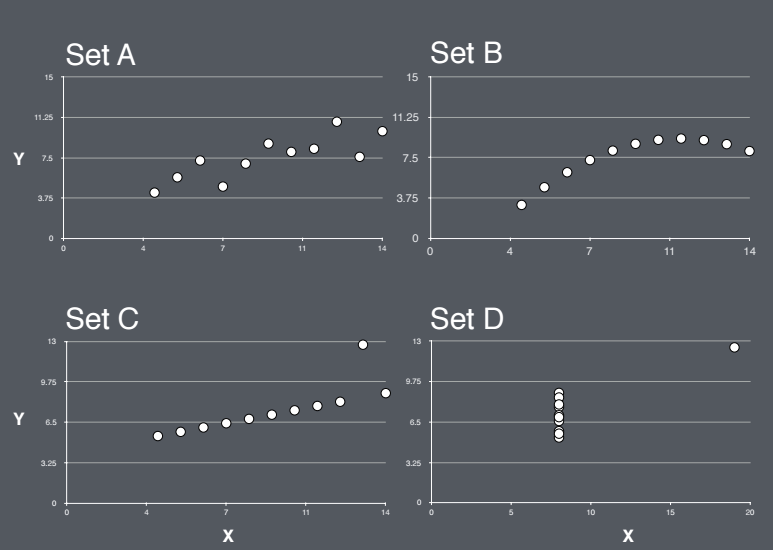
\includegraphics[width=0.5\textwidth]{figures/figure1.png}
    \caption{
      Anscombe's Quartet, a dataset constructed in (Anscombe 1973) to show why graphing data is important}
    \label{fig:example_figure}
  \end{center}
\end{figure}

\subsection{What makes a good visualization?}

In the making of any good visualization, there are several decisions that need to be made. These decisions can have a large effect on the utility of the visualization. A good way to understand what makes a good visualization are two specific design principles, outlined in visualization literature

\begin{itemize}
  \item Expressiveness, can be defined as the extent to which the visualization expresses all the facts in the dataset, and only the facts. Certain visualizations cannot express all the facts of certain kinds of datasets, for example a horizontal dot plot cannot fully express the information of a one-to-many relations dataset. Additionally, expressiveness means not expressing facts that aren't true. {\it Tell the truth and nothing but the truth.}
  \item Effectiveness, measured by how readily the information conveyed is perceived, relative to other visualizations. {\it If the visualization is an encoding, how quickly and accurately can it be decoded by viewers.}
\end{itemize}


\subsection{Steven's Power Law}

\begin{itemize}
  \item $S=I^{P}$, where S is the perceived sensation, I is physical intensity, and P is an empirally determined exponent that varies based on the way the data is conveyed
  \item What this means in terms of data visualization is that different ways to convey the same numerical values of data result in different forms of bias when perceived by humans. The closer the exponent P is to 1 for a way to convey data, the more linear the relationship is, making it a better. For example length is preferable to area when showing the relative size of different quantities.
  \item Effectiveness of different encodings to visualize data have been extensively researched, such as by Cleveland and McGill which compared different porportionality estimates across spatial encodings (position, length, and angle) and the bias associated with them when perceived graphically by users.
  \item Crowdsourced and in-person studies generally show the same results for effectiveness of data visualizations, making crowdsourcing a cheap and effective alternative to traditional studies.

\end{itemize}

\subsection{Additional Data Stuff}

\begin{itemize}
  \item Three main data types: Quantiative (i.e Position, Length, Area), Ordinal (i.e Texture, Slope, Shape--anything that is categorical but where the data has a natural and intuitive ordering scheme), and Nominal (i.e Color)--which is categorical but with no natural ordering. 
  \item Color is an important consideration, important to take into account color blindess, distinguishability, and also black and white printing (when the colors are transferred to grayscale)

\end{itemize}

\subsection{Tools}
\begin{itemize}
  \item There is a tradeoff between speed and expressiveness, where the most fast tools for data visualization are Excel, Google Charts, etc. that are very user-friendly. 
  \item For developers, data scientists, etc., more expressive tools are libraries like D3, ggplot, etc. Most extreme end are graphical libraries like OpenGL, DirectX which can be used to make never-before-seen visualizations
  \item Main categories of tools are Chart Typologies, Declarative Encoding Languages, Component Model Architectures, and Graphics APIs (in order from least to most expressive)
  \item {\it Declarative Langauges} (as opposed to imperative) focus on what you want from execution, rather than the logical steps (how to execute it). 
  \item {\it Wilkinson's Grammar of Graphics} which is a theoretical foundation for producting pretty much all visualizations of data, which has inspired libraries such as D3 and ggplot. Outlines a pipeline for the production of graphics, and also discusses Algebraic foundation (Sets, Operators and Rules) for producing such graphics

\end{itemize}



\section{ggplot2}

In this section of the lecture we went over how to practically use ggplot for data visualizations. The Jupyter notebook that corresponds to the lecture material can be found \href{https://github.com/jhofman/msd2017/blob/master/lectures/lecture_5/visualization_with_ggplot2.ipynb}{HERE} (click for link). These notes serve as a companion to the Jupyter notebook with important points that were mentioned in class regarding using ggplot during the demonstration.

\begin{itemize}
  \item Visualization is {\it always} about communication something. If you are producting visualizations for research for example, you might be trying to communicate a point to readers with each graph. It is important to keep that point in mind when producing these graphics, as way to shape the decisions you make. Similarly, exploratory data analysis is about communicating a point to yourself. 
  \item Some helpful libraries are $lubridate$, which helps with dates, $scales$ which helps make good scales, and $theme\_set$, which helps change color schemes.
  \item ggplot is an implementation of the ideas developed by Wilkinson's {\it Grammar of Graphics}
  \item It is important to pay attention {\it warnings} in ggplot. ggplot may do things for you, such as automatically determining the numbers of bins, but this can in some cases be very unreliable, so it is a best practice to always address the warnings. 
  \item can use pipe to pass things into ggplot, but when you're using ggplot you need to use a plus instead of a pipe
  \item Tip: When using a log scale, it's a good idea to use intervals of 1 and 3
  \item Important to know the difference between $coord\_cartesian$ and $x\_lim$ to know which you actually want to use
  \item Always be sure to $ungroup()$
  \item Facets can be helpful at times, and not helpful at other times. They allow you to view the same type of plot for different data. 


\end{itemize}


\end{document}

%%% Local Variables:
%%% mode: latex
%%% TeX-master: t
%%% End:
